%%%%%%%%%%%%%%%%%%%%%%%%%%%%%%%%%%%%%%%%%%%%%%
% Head matter - can we try to be consistent on
% included packages
 \pdfminorversion=4
\documentclass{beamer}
% \usepackage{amssymb}
% \usepackage{pifont}
% \newcommand{\cmark}{\ding{51}}%
% \newcommand{\xmark}{\ding{55}}%
\mode<presentation>
{\usetheme{default}
 \usecolortheme{default}
 \usefonttheme{default}
 \setbeamertemplate{navigation symbols}{}
 \setbeamertemplate{caption}[numbered]} 
 
\setbeamertemplate{footline}[frame number]
% \usepackage{tabu}
\usepackage[english]{babel}
%\usepackage[utf8x]{inputenc}
\usepackage{amsmath}
\usepackage{multirow}

\usepackage{color,colortbl}
\definecolor{Gray}{gray}{0.85}
\definecolor{LightCyan}{rgb}{0.88,1,1}
\usepackage{booktabs}
% \usepackage[dvipsnames]{xcolor}
\usepackage{amsfonts}
\usepackage{subfig}

\usepackage{mathtools}
\usepackage{bbding}
\usepackage{caption}
\usepackage{tipa}

\usepackage{bm}
\usepackage[export]{adjustbox}
\usepackage{graphicx}
%%%%%%%%%%%%%%%%%%%%%%%%%%%%%%%%%%%%%%%%%%%%%%
% Formatting for title page 
\title{How Phonotactics Affect Multilingual and Zero-shot ASR Performance}
\author{Siyuan~Feng$^{1\dagger}$,
Piotr~\.Zelasko$^{2,3\dagger}$, 
Laureano~Moro{-}Vel{\'{a}}zquez$^{2}$,
Ali~Abavisani$^{4}$, 
Mark~Hasegawa-Johnson$^{4}$, Odette~Scharenborg$^{1}$, Najim~Dehak$^{2,3}$ }
\institute{$^1$Multimedia Computing Group, Delft University of Technology\\ $^2$Center for Language and Speech Processing, $^3$ Human Language Technology Center of Excellence, Johns Hopkins University\\ $^4$Department of Electrical and Computer Engineering, University of Illinois at Urbana-Champaign. ($^{\dagger}$Equal contribution)}
\date{ICASSP 2021, Toronto, Canada (online)\\April 2021}
\newif\ifplacelogo
\placelogotrue
% declare and use the CUHK logo, Optional
%\pgfdeclaremask{cu}{pic-cu-logo-mask}
%\pgfdeclareimage[mask=cu,width=4cm]{cu-logo}{pic-cu-logo-en-ch}
%\logo{\vbox to 0.65cm{\hbox to 10cm{\hfil\pgfuseimage{cu-logo}}}}
% \titlegraphic{\vspace{0.5cm}\hspace*{0.5cm}\includegraphics[height=0.8cm]{dsp_logo.png}\hspace*{3cm}\includegraphics[height=0.8cm]{pic-cu-logo-en-ch.png}}
%\logo{\includegraphics[height=0.8cm]{pic-cu-logo-en-ch.png}\vspace{10pt}}
%%%%%%%%%%%%%%%%%%%%%%%%%%%%%%%%%%%%%%%%%%%%%%
\begin{document}
\begin{frame}[noframenumbering,plain]
  \titlepage
\end{frame}
\begin{frame}[noframenumbering,plain]{Outline}
\tableofcontents
    
\end{frame}
 
\section{Introduction}
% \begin{frame}{Introduction}
% \framesubtitle{Ultimate goal}
% \begin{block}{ASR for unwritten languages}
% \begin{itemize}
%     \item Only 
% \end{itemize}
% \end{block}
    
% \end{frame}

\begin{frame}{Introduction}
\framesubtitle{Our goal: ASR for low-resource languages}
% \cite{Zelasko2020That}
% Utimately, we 

 ASR  for  low-resource languages is challenging:
\begin{itemize}
    \item Lack of transcribed data, lexicons available.
    % \item 
    % \item
\end{itemize}
Crosslingual knowledge transfer can help:
\begin{enumerate}
    \item Pretraining (non-target languages) $\rightarrow$ fine-tuning (target language).
    \item Multilingual training: language-dependent phone sets.
    \item Multilingual training: a language-independent (universal) phone set.
\end{enumerate}
\begin{block}{}
\textbf{Multilingual training is beneficial to low-resource languages.}
\end{block}

\end{frame}

\begin{frame}{Introduction}
\framesubtitle{Insights into multilingual AM training}
    % The advantage of multilingual AM training is probably due to phonetic representation sharing across languages.\\
    % However past research merely reported  overall phone/word error rate reduction.
    Why is multilingual AM training useful?
    \begin{itemize}
        \item Phonetic representation sharing across languages.
        \item More training data.
        \item Multilingual training acts as regularization.
        % \item Most  research only reported  overall phone/word error rate reduction, without analysis.
        % \item \textcolor{blue}{What aspects of phonetic representations a multilingual AM learns?}
        % \item \textcolor{blue}{Is multilingual AM equally benefiting every phone unit?}
    \end{itemize}
    It is unclear: 
    \begin{itemize}
        \item What aspects of the phonetic representations a multilingual AM learns?
        \item Is multilingual AM equally benefiting every phone unit?
        \item  Most  research only reported  overall phone/word error rates without analysis.
    \end{itemize}
   
\end{frame}
\begin{frame}{Introduction}
\framesubtitle{Recent study on analyzing multilingual AM}
\cite{Zelasko2020That_interspeech}\footnote{That sounds familiar: an analysis of phonetic representations transfer across languages. \textit{In Interspeech 2020.}}  performed an analysis of multilingual AM training:
\begin{itemize}
    \item Adopted an encoder-decoder ASR architecture.
    \item Performed  universal phone-level ASR and   analysis.
    % \item Found that: 
\end{itemize}
Observation:
\begin{itemize}
    % \item All phones (incl. language-unique ones) benefit from multilingual training (versus monolingual); 
    \item Phonetic representations less effective in transferring to an \textbf{unseen language} than to  a seen language.
    \item Unseen language: test language not included during model training - \textbf{zero-shot learning}.
\end{itemize}

\end{frame}
\begin{frame}{Introduction}
\framesubtitle{Motivation of current study}
% A question raised by \cite{Zelasko2020That_interspeech}: \\
Why does multilingual ASR perform much worse on unseen languages?
\begin{itemize}
    \item Differences in  \textcolor{black}{pronunciation}, or  mismatch in language \textcolor{black}{phonotactics}? 
    \item \cite{Zelasko2020That_interspeech} did not answer, because acoustics and phonotactics are modeled within a single e2e model.
\end{itemize}

% It is not possible to find answers in \cite{Zelasko2020That_interspeech}, as:
% \begin{itemize}
%     % \item 
%     % \item Pronunciation: AM.
%     % \item Phonotactics: 
%     \item In an encoder-decoder ASR architecture, \textcolor{black}{acoustics} and \textcolor{black}{phonotactics} are modeled within a single model.
%     % \item 
% \end{itemize}

\begin{block}{}
\textbf{In the current work:}
\begin{itemize}
    \item Investigate the role of phonotactics on phone-level ASR performance.

    \item Adopt the hybrid ASR architecture.
    \item Hybrid ASR systems model acoustics and phonotactics in AM and LM separately.
    % \item 
\end{itemize}
    
\end{block}

\end{frame}
 
\section{Experimental setup}
\begin{frame}{Experimental setup}
\framesubtitle{Experiment design}

\begin{block}{Task: IPA\footnote{International Phonetic Alphabet.} phone recognition.}
\begin{itemize}
    \item Every phone is represented by IPA symbol(s), irrespective of the language: i.e. a universal phone representation.
    \item Convert speech sentences into  IPA phone sequences. 
\end{itemize}
\end{block}
\begin{block}{Language coverage}
\begin{itemize}
    \item $13$ languages from two corpora.
    \item GlobalPhone \cite{Schultz02globalphone}: Czech, French, Spanish, Mandarin, Thai; $11\sim 24$ hours of training data/language.
    \item Babel: Cantonese, Bengali, Vietnamese, Lao, Zulu, Amharic, Javanese, Georgian; $39\sim 127$ hours of training data/language.
\end{itemize}

\end{block}
    
\end{frame}
\begin{frame}{Experimental setup}
\framesubtitle{Experiment design}
\begin{block}{Three AM training scenarios}
\begin{enumerate}
    \item Monolingual - baseline.
    \item Multilingual 
           \begin{itemize}
            \item $13$ languages in training, tested on each language.
        \end{itemize}
    \item \textbf{Crosslingual} (\textbf{zero-shot})
    \begin{itemize}
            \item $12$ languages in training, tested on the remaining $1$ language.
            \item Investigate if universal phone representations exist that can be used for unseen language ASR.
        \end{itemize}
\end{enumerate}
     
\end{block}


    
\end{frame}
\begin{frame}{Experimental setup}
\framesubtitle{Experiment design}

\begin{block}{Phonotactic and word LMs}
Measure the effect of phonotactics in the phone-level ASR performance:
 \begin{itemize}
     \item Phonotactic LMs of uni-, bi- and tri-gram (\textbf{ug, bg, tg}).
     \item Word LM of tri-gram (\textbf{wtg}).
     \item Amount of phonotactic information: ug $<$ bg $<$ tg $<$ wtg.
 \end{itemize}
 Each mono/multi/crosslingual AM is scored with ug, bg, tg and wtg separately.
    
\end{block}
    
\end{frame}
\begin{frame}{Experimental setup}
\framesubtitle{Implementation}
\begin{block}{Word- to phone-level transcription conversion}
LanguageNet G2P models \cite{hasegawa2020grapheme}.
    
\end{block}
\begin{block}{Hybrid DNN-HMM AM}
\begin{itemize}
    \item $12$-layer TDNNF network, trained using Kaldi \cite{povey2011kaldi}.
    \item Training criterion: LF-MMI.
    \item Input: $43$-D MFCC+pitch  and $100$-D i-vector.
    \item Identical TDNNF structure for mono/multi/crosslingual experiments.
    \item $13$ monolingual AMs, $1$ multilingual AM, $13$ crosslingual AMs. ($13$ languages)
\end{itemize}

\end{block}    
\end{frame}
\begin{frame}{Experimental setup}
\framesubtitle{Implementation}
\begin{block}{Phonotactic and word LMs}
\begin{itemize}
    % \item Estimated using SRILM \cite{Stolcke02srilm--}.
    \item Trained with phone-level and word-level transcripts respectively, using  SRILM \cite{Stolcke02srilm--}.
    \item Depending on the training scenario, a LM is trained with 
        \begin{itemize}
            \item $1$ language:  mono-ug/-bg/-tg/-wtg.
            \item $13$ languages: multi-ug/-bg/-tg/-wtg.
            \item $12$ languages: cross-ug/-bg/-tg/-wtg (the target language is not used during training of the LMs).
        \end{itemize}
    % $1$ (mono-ug/-bg/-tg/-wtg) or $13$ (multi-ug/-bg/-tg/-wtg) or $12$ (cross-ug/-bg/-tg/-wtg) languages' data.
    % \item Word LM trained with 
\end{itemize}
    
\end{block}


    
\end{frame}
\begin{frame}{Experimental setup}
\framesubtitle{Implementation}
\begin{block}{Scoring an AM with different LMs}
\begin{enumerate}
    \item Monolingual AM: mono-ug/-bg/-tg/-wtg.
    \item Crosslingual (zero shot) AM: cross-ug/-bg/-tg/-wtg, and (test language) mono-tg.
        \begin{itemize}
            \item Mono-tg allows for checking AM transferability  alone.
            \item Mono-tg does not represent a zero-shot scenario.
        \end{itemize}
    \item Multilingual AM: multi-ug/-bg/-tg/-wtg, and (test language) mono-tg/-wtg.
        \begin{itemize}
            \item Mono-tg/-wtg versus multi-tg/-wtg allows for measuring the effect of imposing non-target language phonotactics in phone ASR.
        \end{itemize}
\end{enumerate}
%     \item 
% \end{itemize}
    
\end{block}
    
\end{frame}
\section{Experimental results}
\begin{frame}{Experimental results}
\framesubtitle{Comparison of AMs}
 

 
\begin{columns}
    \column{0.4\linewidth}
    % Phonotactic LM: mono-tg.
    \begin{table}
\renewcommand\arraystretch{0.6}
\centering
\caption{PER ($\%$) results  under Mono/cross/multilingual scenarios.    $^{\ddagger}$ indicates tone languages.}
\resizebox{   \linewidth}{!}{%
\begin{tabular}{l|ccc}      
% \hline      
\toprule
 AM & Mono  & Cross   & Multi   \\
 \midrule
%  AM & Mono & \multicolumn{4}{c}{Cross} & \multicolumn{4}{c}{Multi}  \\
LM  & \multicolumn{3}{c}{Mono-tg}    \\
\midrule
Czech &14.1&  55.2 & 18.6 \\%11.0\\
French & 16.7 & 55.1 & 19.9\\
Spanish & 10.3 & 33.9 &11.2\\
Mandarin$^{\ddagger}$  &  17.6 & 80.4 & 21.0\\ 
Thai$^{\ddagger}$  & 18.8 & 73.6&27.5\\
\midrule
Cantonese$^{\ddagger}$  & 39.8 & 87.6 &42.9\\
Bengali & 41.1 & 66.8& 43.3\\
Vietnamese$^{\ddagger}$ & 41.6 &87.5&45.8\\
Lao$^{\ddagger}$ & 39.8 &86.5& 43.3\\
Zulu$^{\ddagger}$ & 44.6 & 72.8& 46.1\\
Amharic & 41.6           & 74.8& 45.7\\
Javanese & 48.3          & 69.6& 50.6\\
Georgian & 39.1          & 63.9&39.9\\
% French&22.5&20.3&16.7&\textbf{13.0}&63.1&62.9&64.1&\textbf{55.1}&76.4&27.2&25.4&21.8&19.9&14.4&\textbf{14.3}\\%14.4\\
% Spanish&12.2&11.8&\textbf{10.3}&10.7&56.5&57.2&64.6&\textbf{33.9}&61.4&14.5&12.7&11.1& 11.2 &\textbf{11.0}&11.2\\%11.0\\
% Mandarin$^{\ddagger}$&26.9&20.2&\textbf{17.6}&-&87.8&88.2&89.8&\textbf{80.4}&-&43.4&26.1 &\textbf{20.4}&21.0&-&-\\
% Thai$^{\ddagger}$&21.9&20.0&\textbf{18.8}&-&83.3&86.8&88.7&\textbf{73.6}&-&40.2&32.2 &\textbf{27.2}&27.5&-&-\\
% \midrule
% Cantonese$^{\ddagger}$&61.2&44.7&39.8&\textbf{34.8}&91.2&90.8&91.0&\textbf{87.6}&90.8&75.9&55.2&43.6&42.9&39.1&\textbf{38.8}\\%39.1\\
% Bengali&59.8&46.9&41.1&\textbf{41.0}&86.0&83.1&81.3&\textbf{66.8}&87.7&67.9&56.1 &45.6&\textbf{43.3}&44.5&43.7\\%44.5\\
% Vietnamese$^{\ddagger}$&54.2&45.0&\textbf{41.6}&42.6&92.5&91.5&91.1&\textbf{87.5}&94.4&67.8&51.3&\textbf{45.8}&\textbf{45.8}&47.7&46.8\\%47.7\\
% Lao$^{\ddagger}$&66.6&46.4&\textbf{39.8}&41.8&87.2&\textbf{85.9}&86.0&86.5&92.7&72.4&56.6 &45.1&\textbf{43.3}&48.3&46.2\\%48.3\\
% Zulu$^{\ddagger}$&70.6&54.1&44.6&\textbf{40.5}&86.3&83.5&82.3&\textbf{72.8}&86.0&72.2&59.7&47.9&46.1&45.3&\textbf{44.4}\\%45.3\\
% Amharic&61.2&49.3&41.6&\textbf{32.7}&87.2&83.4&81.0&\textbf{74.8}&82.2&72.7&61.1 &50.2&45.7&39.2&\textbf{38.2}\\%39.2\\
% Javanese&57.6&52.3&48.3&\textbf{45.3}&87.0&84.6&85.0&\textbf{69.6}&87.4&65.1&60.9 &56.8&50.6&53.3&\textbf{49.9}\\%53.3\\
% Georgian&52.8&42.9&39.1&\textbf{34.6}&85.5&81.4&80.0&\textbf{63.9}&86.8&60.4&48.4 &42.4&39.9&38.8&\textbf{37.3}\\%38.8	\\
\bottomrule
\end{tabular}%
% \footnotetext{`speakers-R/-L' denotes speakers with rich/limited speech data}
}
\label{tab:PER_results_am}
\end{table}
    \column{0.6\linewidth}
    \begin{footnotesize}
        \begin{block}{}
           Phonotactic LM: mono-tg.
        \end{block} 
        \begin{block}{Observations}
        \begin{itemize}
            \item Crosslingual AM consistently the worst.
            \item Monolingual AM better than multilingual AM. Possible explanation: too many  ($\sim 800$) shared phones across $13$ languages.
        \end{itemize}
    
    \end{block}
    \end{footnotesize}

\end{columns}
    
\end{frame}
\begin{frame}{Experimental results}
\framesubtitle{Effect of phonotactics: multilingual ASR}
\begin{columns}
    \column{0.5\linewidth}
        \begin{table}
\renewcommand\arraystretch{0.6}
\centering
\caption{PER ($\%$) results  under the multilingual scenario.   }
\resizebox{   \linewidth}{!}{%
\begin{tabular}{l|cc|cc}      
% \hline      
\toprule
 AM & \multicolumn{4}{c}{Multi}   \\
 \midrule
%  AM & Mono & \multicolumn{4}{c}{Cross} & \multicolumn{4}{c}{Multi}  \\
LM type & \multicolumn{2}{c|}{Phonotactic} & \multicolumn{2}{c}{Word} \\
LM  & Multi-tg & Mono-tg & Multi-wtg & Mono-wtg    \\
\midrule
Czech &28.8 &  18.6  & 11.0 &9.5 \\%11.0\\
French &  27.2 & 19.9  &14.4 &14.3\\
Spanish & 14.5  & 11.2  &11.0&11.2\\
Mandarin$^{\ddagger}$  & 43.4  & 21.0  &-&-\\ 
Thai$^{\ddagger}$  &40.2  &27.5  &-&-\\
\midrule
Cantonese$^{\ddagger}$  &75.9   & 42.9  &39.1&38.8\\
Bengali &67.9   & 43.3 &44.5 &43.7\\
Vietnamese$^{\ddagger}$ &67.8  &45.8 &47.7&46.8\\
Lao$^{\ddagger}$ & 72.4 &43.3 & 48.3&46.2\\
Zulu$^{\ddagger}$ &72.2   & 46.1  &45.3 &44.4\\
Amharic &72.7             & 45.7 &39.2 &38.2\\
Javanese &65.1            & 50.6 & 53.3& 49.9\\
Georgian &60.4            & 39.9 &38.8&37.3\\
 
\bottomrule
\end{tabular}%
% \footnotetext{`speakers-R/-L' denotes speakers with rich/limited speech data}
}
\label{tab:PER_results_lm1}
\end{table}
    \column{0.5\linewidth}
    \begin{footnotesize}
        AM: Multilingual TDNNF.
        \begin{block}{Observations}
            \begin{itemize}
                \item Mono-tg better than Multi-tg; 
                \item Mono-wtg better than Multi-wtg in most languages.
                \item word LM better than phonotactic LM.
            \end{itemize}
        \end{block}
        \begin{block}{Conclusion}
            \begin{itemize}
                \item Non-target language phonotactics is harmful for phone-level ASR in a target language.
                \item Multilingual ASR benefits from imposing stronger phonotactics in the target language. 
            \end{itemize}
            
        \end{block}
    \end{footnotesize}
\end{columns}
    
\end{frame}
\begin{frame}{Experimental results}
\framesubtitle{Effect of phonotactics: crosslingual (zero-shot) ASR}
    \begin{columns}
        \column{0.45\linewidth}
        \begin{table}
\renewcommand\arraystretch{0.6}
\centering
\caption{PER ($\%$) results  under the crosslingual (zero-shot) scenario. }
\resizebox{   \linewidth}{!}{%
\begin{tabular}{l|cc|c}      
% \hline      
\toprule
 AM & \multicolumn{3}{c}{Cross}   \\
 \midrule
%  AM & Mono & \multicolumn{4}{c}{Cross} & \multicolumn{4}{c}{Multi}  \\
LM  & Cross-wtg & Cross-tg & Mono-tg    \\
\midrule
Zero-shot & Yes &  Yes & No \\
\midrule
Czech &    78.2  & 70.5  & 55.2 \\%11.0\\
French &     76.4   & 64.1 & 55.1\\
Spanish &   61.5  & 64.6& 33.9 \\
Mandarin$^{\ddagger}$  &-      & 89.8& 80.4\\ 
Thai$^{\ddagger}$  &    -  & 88.7 & 73.6 \\
\midrule
Cantonese$^{\ddagger}$  & 90.8  & 91.0&87.6 \\
Bengali & 87.7  & 81.3& 66.8\\
Vietnamese$^{\ddagger}$ & 94.4  &91.1&87.5\\
Lao$^{\ddagger}$ &92.7 &86.0&86.5 \\
Zulu$^{\ddagger}$ & 86.0 &82.3&72.8\\
Amharic &   82.2    &81.0&74.8  \\
Javanese &  87.4   &85.0&69.6  \\
Georgian &  86.8     &80.0&63.9  \\
 
\bottomrule
\end{tabular}%
% \footnotetext{`speakers-R/-L' denotes speakers with rich/limited speech data}
}
\label{tab:PER_results_lm2}
\end{table}
\column{0.55\linewidth}
\begin{footnotesize}
    \begin{block}{Observations}
    \begin{itemize}
        \item  Mono-tg better than Cross-tg and Cross-wtg.
        \item  Cross-tg better than Cross-wtg.
    \end{itemize}
    
\end{block}
\begin{block}{Conclusion}
    \begin{itemize}
        \item Phonotactic information of the target language (in Mono-tg) is crucial.
        \item Too strong phonotactic constraint (Cross-wtg comparing to Cross-tg) from other languages is harmful to phone ASR for a target language.
    \end{itemize}
\end{block}
\end{footnotesize}

    \end{columns}
\end{frame}


\section{Discussion}
% \begin{frame}{Discussion}
% \framesubtitle{Breakdown of PER results}
% \begin{table}[t]
% \renewcommand\arraystretch{0.8}
%     \centering
%      \resizebox{0.5\linewidth}{!}
%       {
%     \begin{tabular}{ccrrrr}
%     \toprule
%     AM    & LM        & PER & Ins. & Del. & Sub. \\
%     \midrule
%     Mono  & mono-wtg  & 30.0 & 17.6 & 34.0 & 48.4 \\
%     Mono  & mono-tg   & 37.7 & 11.5 & 39.6 & 48.9 \\
%     Multi & multi-wtg & 34.2 & 18.3 & 29.2 & 52.5 \\
%     Multi & multi-tg  & 43.0 &  9.6 & 40.2 & 50.3 \\
%     Cross & cross-wtg & 85.1 &  3.2 & 40.6 & 56.1 \\
%     Cross & cross-tg  & 82.6 &  2.3 & 42.1 & 55.6 \\
%     \bottomrule
%     \end{tabular}
%     }
%     \caption{PERs ($\%$) computed across all languages for mono/multi/crosslingual systems and their breakdown into three error types: Insertion, Deletion and Substitution.}
%     \label{tab:error_fraction}
% \end{table}
% \begin{block}{}
%     \begin{footnotesize}
%     \begin{itemize}
%         \item Substitutions dominate.
%         \item Large number of Deletions.
%     \end{itemize}
%     \end{footnotesize}

% \end{block}
    
% \end{frame}
 \begin{frame}{Discussion}
 \framesubtitle{Distribution of PER for different phones.}
 \begin{figure}
     \centering
     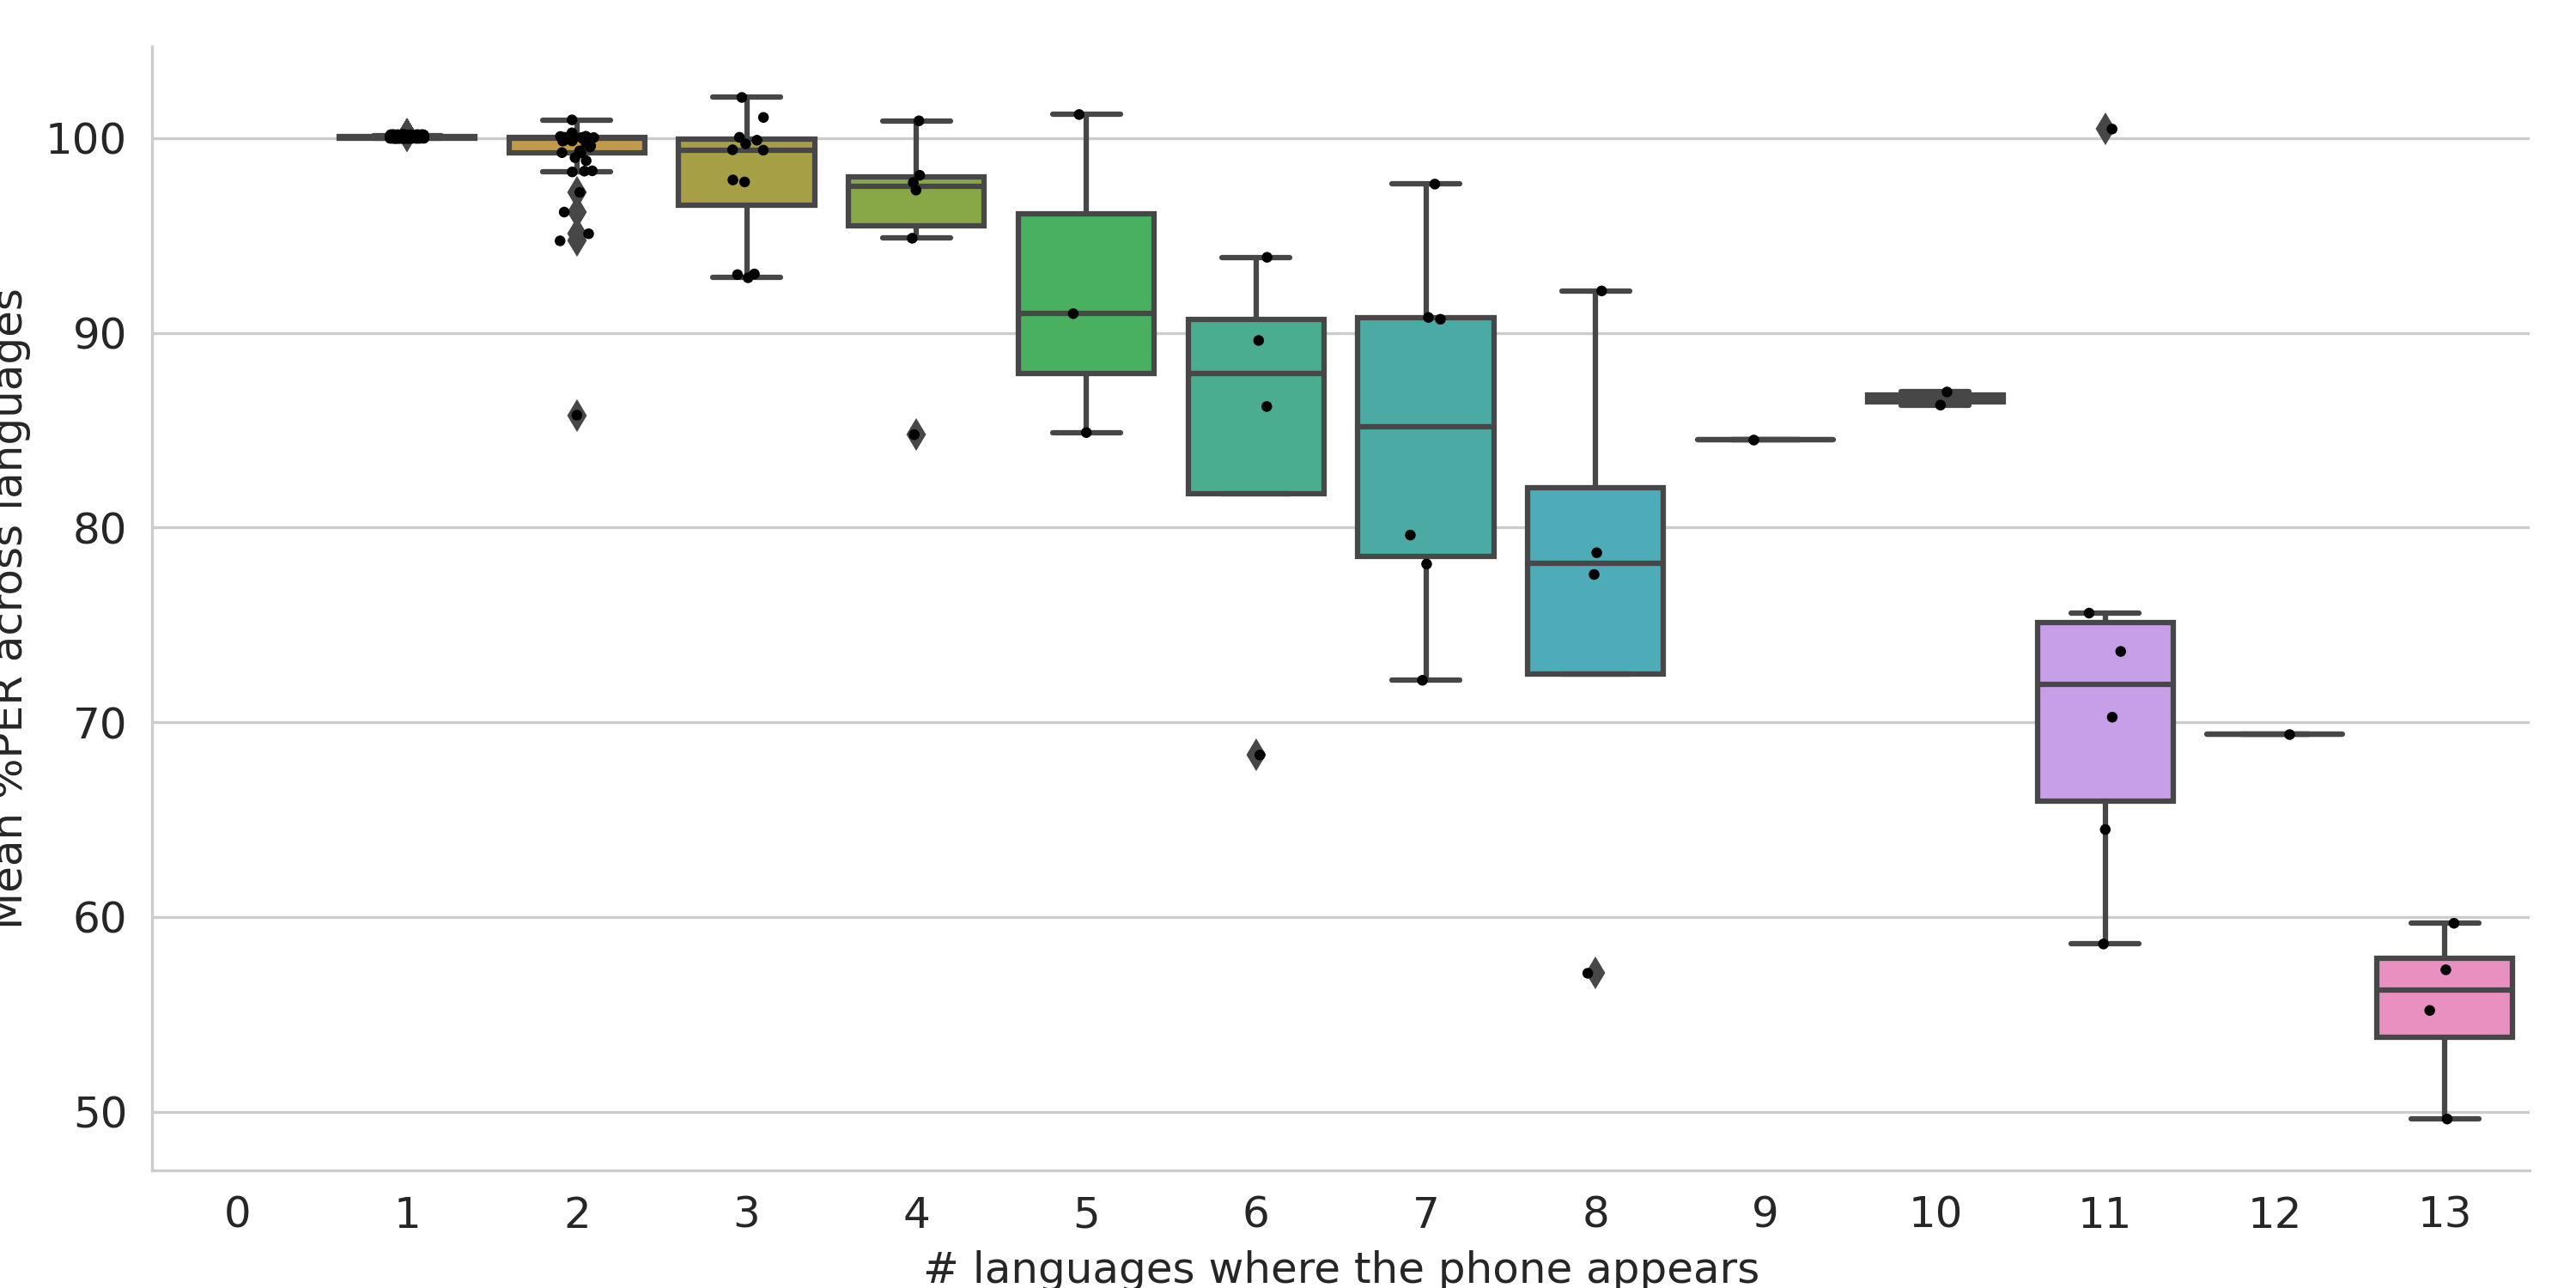
\includegraphics[width=0.6\linewidth]{Figure/per_language_per_crosslingual.png}
     \caption{Distribution of PERs for different phones, depending on how many languages share that phone. PERs are computed in the crosslingual experiments.}
     \label{fig:distr_phone}
 \end{figure}
 \begin{block}{}
     \begin{footnotesize}
            \begin{itemize}
                \item Phones existing in more languages have lower PER in zero-shot ASR experiments.
                \item Consistent with findings in E2E ASRs \cite{Zelasko2020That_interspeech}, suggesting this is universal across ASR architectures.
                % \item 
            \end{itemize}
     \end{footnotesize}
 \end{block}
     
 \end{frame}
 \begin{frame}{Summary}
% \framesubtitle{Summary}
\begin{itemize}
    \item In the multilingual ASR task, systems benefit from imposing stronger phonotactics of the target language.
    \item In the zero-shot ASR task, too strong phonotactics is harmful. Suggestion:  build an LM  at the phone level rather than at the word level, when leveraging non-target languages.
    % \item 
    \item In both the multilingual and the zero-shot ASR tasks, using non-target languages' phonotactics in LM  training is  harmful to phone recognition for a target language.
\end{itemize}
    
\end{frame}
% \section{References}
\begin{frame}[allowframebreaks,noframenumbering,plain]{References}
%\bibliographystyle{IEEEtran}
\bibliographystyle{apalike}
\begin{tiny}
\bibliography{refs}
\end{tiny}
\end{frame}



\end{document}
